\chapter{Continuous modeling of the membrane dynamics}

\label{continuous_model_description}

The stochastic approach to the biophysical systems described in the previous chapters (Monte-Carlo simulations), due to a significant computational cost, can only be used when the number of particles $N$, involved in the simulation, is low. Moreover, to faithfully describe the system evolution it is necessary to take into account the interactions of all particles with each other. This detailed description does not allow to significantly increase the size of the system. As shown in the previous chapters, it is only possible to simulate the system behavior at the nano- scale. To simulate an evolution of the system at scales of several micrometers one has to turn to another modeling approximation which is computationally suitable for systems of this size. One particularly effective and commonly used approach is the continuous deterministic framework, which has been extensively used in earlier studies of membrane dynamics \cite{May2000,Khelashvili2008}. This framework is only applicable to systems with a large number of particles $N$ (comparable to $N_A = 6.02\cdotp10^{23}$ 1/mol). The concentration of particles in such a system can be approximated by a continuous function. The behavior of this function is governed by initial conditions, system parameters and by a differential equation. Since the solution of any differential equation with fixed parameters is always determined by initial conditions, the framework is deterministic. The continuous deterministic approach is very fast and computationally efficient, allowing one to work at big (micrometer) scales. The system of differential equations, which describes the behavior of all system components, can be derived from a stochastic description of the same system in the continuous (mean-field) limit, i.e. when $N$ becomes infinitely large. In this case the system noise vanishes, since relative fluctuations typically decrease as $\sqrt{N}$ ($\lim_{N\to\infty}\sqrt{N}/N = 0$).

To extend the model of peptide-membrane dynamics to larger scales I will use such a continuous deterministic approach. Below I describe how the continuous model (CM abbreviation is used throughout the text) of the system is constructed and implemented.

\section{Membrane model}

The peptide-membrane system is defined in the same way as in the MCA (chapter \ref{Monte_Carlo_model_description}), except three major modifications. First, I assume that the lipids and the peptides diffuse in the same plane (membrane plane hereafter). This simplification is sensible due to the fact that in the mean-field approximation the particles can be infinitely close to each other. Second, instead of a single peptide, there is a large number of peptides in the CM, diffusing in the membrane plane. Finally, the membrane plane is not discretized as it was in the MCA, instead the number of lipids and peptides at any point of the plane is defined by their concentrations.

\subsection{Membrane plane in the absence of peptides}

First, I begin the construction of the CM with a description of the membrane plane in the absence of peptides. In this case the membrane plane consists of lipid head groups of 3 lipid species (PS, PIP$_2$ and PC) with corresponding concentrations $c_i$ ($i\in[1,3]$) and charges $z_i$. The cytoplasmic solution is chosen to be the same as was used in the MCA: 0.1 M of 1:1 electrolyte with concentrations of positive and negative ions $n_+$ and $n_-$, correspondingly. The concentrations of lipids and mobile ions are smooth functions of distance $\vec{\mathbf{r}}$ in a 2D space and they are defined in every point of the membrane plane. The behavior of these functions is described by a system of differential equations. The equations are usually dictated by physical properties of the system. In order to derive them I use a universal thermodynamical approach. In this approach a free energy $F$ of a closed system is introduced, which measures a ``useful'' work obtainable from the system at constant temperature and volume. I assume that the system has a constant volume and is in thermodynamic equilibrium with a heat bath at absolute temperature $T$ = 298 K. To obtain the mean-field approximation of the system one has to minimize $F$ \cite{Chaikin2000}. Minimization of F provides important thermodynamical characteristics of the system, such as electro-chemical potentials and distributions of system components. Based on these characteristics one can derive a system of differential equations, which describes the behavior of all components.

\subsection{Free energy}

I start with the definition of a free energy. In thermodynamics a free energy (or Helmholtz free energy) of a closed system at temperature $T$ and volume $V$ is defined as follows:
\begin{equation}
 \label{free_energy}F=U-TS
\end{equation}
where $U$ is the internal energy of the system, $T$ is the absolute temperature (in Kelvin) and $S$ is the entropy of the system. Alternatively, the free energy can be represented by means of a free energy density:
\begin{equation}
 \label{free_energy_density}F=\int_V f dv=\int_V (u-Ts)dv
\end{equation}
where $u$ and $s$ are an internal energy density and an entropy density, correspondingly. In contrast to the free energy $F$, the free energy density $f$ is not an integral characteristics of the whole system, but instead it is defined at every point $\vec{\mathbf{r}}$ of the membrane. I will use $f$ for deriving an expression of the free energy $F$.

\subsection{Entropy density}

\label{entropy_density}

I begin a detailed description of the free energy \eqref{free_energy_density} with the definition of the entropy (or entropy density). Entropy density is an essential property of any system and it reflects the number of ways in which a system may be arranged. Alternatively, it is a measure of disorder in the system. In order to find an analytical expression of the entropy density I use a statistical mechanics approach. Statistical mechanics describes properties of particle ensembles under different conditions. To analyze the ensemble properties statistical mechanics provides a powerful tool: a partition function. The partition function is introduced to describe thermodynamic properties of a system in equilibrium. The key feature of the partition function is that most of thermodynamic properties of the system, such as the internal energy $U$, the free energy $F$ or the entropy $S$ can be expressed in terms of the partition function or its derivatives. To derive an expression of the entropy density I use a partition function of the so-called canonical ensemble \cite{Huang1963}:
\begin{equation}
\label{partition_function} Z_N=\int \frac{d^{3N}p\hspace{0.1in}d^{3N}q}{N!h^{3N}}e^{-\beta \hat{H}(p,q)}
\end{equation}
where $p$ and $q$ are momenta and coordinates of particles in the ensemble, $N$ is the total number of particles in the ensemble, $\hat{H}$ is a Hamiltonian of the ensemble, $h$ is a constant of the dimension of momentum$\times$distance (Planck's constant) and $\beta = 1/(k_BT)$, $k_B$ is the Boltzmann's constant. 

The partition function shows the volume in ($p,q$) space, occupied by the ensemble. The pre-exponent term in eq. \eqref{partition_function} defines the total number of states in ($p,q$) space, available for the ensemble to occupy. $1/N!$ factor in this term is the so-called ``correct Boltzmann counting'' factor. It was introduced by Gibb's to resolve Gibb's paradox. The paradox refers to the fact that without this factor in the partition function, the entropy of a closed system of two indistinguishable ideal gases decreases, which is in disagreement with the second law of thermodynamics.

The Hamiltonian $\hat{H}$ is, by definition, a total energy of the ensemble. It is defined as a sum of kinetic and potential energies of all particles:
\begin{equation}
 \label{hamiltonian}\hat{H} = \sum_{i=1}^N \frac{p_i^2}{2m} + \hat{U}
\end{equation}

To define the analytical expression of the entropy density $s$ I use eq. \eqref{partition_function} and the definition of the entropy:
\begin{equation}
 \label{entropy_general} S=k_B \log(Z_N)
\end{equation}

It is only possible to analytically compute $S$ using eq. \eqref{entropy_general} if one neglects the potential energy (in the membrane plane I consider only electrostatic interactions between system particles) in the Hamiltonian $\hat{H}$. In this case the computed entropy is the translational entropy of an ideal gas of particles. This approximation is necessary due to the complications appearing in the exact calculations of the potential energy contributions to the partition function. This simplification in computing the entropy of a charged solution has been used in many other works and has been extensively validated \cite{Haleva2004,May2000,Khelashvili2008}. Note that other approximations can be used to account for this issue \cite{Laird1994}.

Using eqs. \eqref{partition_function} and \eqref{hamiltonian} with $\hat{U}=0$ and remembering the integral of the normal distribution ($\int e^{-\frac{x^2}{a}} dx = \sqrt{\pi a}$), the partition function can be written as:
\begin{align}
 \label{partition_function1} Z_N&=\int \frac{d^{3N}p\hspace{0.1in}d^{3N}q}{N!h^{3N}}e^{-\beta \sum_{i=1}^N \frac{p_i^2}{2m}}= \nonumber \\
&= \int e^{-\frac{p_1^2}{2mk_BT}} d^3 p_1 \int e^{-\frac{p_2^2}{2mk_BT}} d^3 p_2 \hspace{0.1in} ... \int e^{-\frac{p_N^2}{2mk_BT}} d^3 p_N \int \frac{d^{3N}q}{N!h^{3N}} = \nonumber \\
&= \frac{(2\pi m k_B T)^{\frac{3N}{2}}}{N!h^{3N}} \int d^{3N}q = \Big(\frac{2\pi m k_B T}{h^2}\Big)^{\frac{3N}{2}}\frac{V^N}{N!} = \frac{V^N}{V_0^N N!}
\end{align}
where $V_0$ is a constant volume $V_0 = \Big(\frac{2\pi m k_B T}{h^2}\Big)^{-\frac{3}{2}} = \frac{1}{\lambda_r^3}$, $\lambda_r$ is the thermal de Broglie wavelength and $V$ is a physical volume occupied by the ensemble. Note that the kinetic energy of particles in the Hamiltonian $\hat{H}$ contributes only as a constant $V_0$ and does not provide any concentration dependence to the entropy.

Substituting eq. \eqref{partition_function1} in the entropy equation \eqref{entropy_general} one can obtain:
\begin{equation}
 \label{entropy_general1}S=k_B\log{\Big(\frac{V^N}{V_0^NN!}\Big)}
\end{equation}

After rearranging the expression under the logarithm in eq. \eqref{entropy_general1}, the entropy density $s=S/V$ will have the form:
\begin{equation}
 s=k_B\Big(\frac{N}{V}\log\Big({\frac{V}{V_0}}\Big) - \frac{1}{V}\log{N!}\Big)
\end{equation}

Application of the Stirling's approximation for large $N$ ($\log{N!} = N \log{N} - N + O(log(N))$) to the equation above yields:
\begin{align}
 s&=k_B\Big(\frac{N}{V}\log\Big({\frac{V}{V_0}}\Big) - \frac{N}{V}\log{N} + \frac{N}{V}\Big)= \nonumber \\
 \label{entropy0}&=-k_B\Big(\frac{N}{V}\log\Big({\frac{NV_0}{V}}\Big) - \frac{N}{V}\Big)
\end{align}

So that \eqref{entropy0} is equivalent to:
\begin{equation}
 \label{entropy}s = -k_B(\rho\log({\rho V_0})-\rho)
\end{equation}
where $\rho$ is a concentration of particles of the ensemble (in 1/m$^3$ units).

Eq. \eqref{entropy} provides an expression of the translational entropy density of the ensemble, which can be used to define a translation entropy density of each species in the membrane plane. Notice also that entropy is an extensive quantity \cite{Chandler1987}, which means that the total entropy of the system is the sum of the entropies of all species. Thus, for the membrane plane under consideration, consisting of 3 lipid species and $n_+$ and $n_-$ cytoplasmic ions, the entropy density will have the following form:
\begin{equation}
 \label{entropy_sum}s = -k_B\Big(\sum_{i=1}^3(c_i\log({c_i V_0})-c_i) + n_+ \log({n_+  V_0}) - n_+ + n_- \log({n_-  V_0}) - n_-\Big)
\end{equation}

\subsection{Internal energy density}

\label{internal_energy}

The second term in the right hand side of the free energy $F$ \eqref{free_energy_density} is the internal energy density $u$. By definition, $u$ is an average total energy density of the ensemble, consisting of the average kinetic and the average potential energy densities. Since for the membrane plane the kinetic energy density is already included in the entropy density $s$ (see subsection \ref{entropy_density}), in $u$ I consider only the contribution of the potential energy density. However, as described above (subsection \ref{entropy_density}), an exact analytical expression of the potential energy density cannot be obtained. To be able to calculate it, the mean-field approximation can be used \cite{Huang1963}. In the mean field approximation particles do not interact directly with each other, instead each of them interacts with a mean potential field created by others. The potential is always defined up to a constant, therefore I assume that the value of the potential is 0 in the infinity.

By definition, in the mean field approximation the main part of the internal energy density $u$ of a static electrical system, consisting of identical ions with charges $q$ and the concentration $\rho$, is defined as a work, required to bring these ions from the infinity to given points, and can be written as: $u=q \rho \phi$, where $\phi$ is a value of the electrostatic potential at the given point. 

If one introduces a non-dimensional electrostatic potential as follows:
\begin{equation}
 \label{potential}\psi = \frac{e\phi}{k_B T}
\end{equation}
where $e$ is the electron charge, then the work $u$ can be rewritten as:
\begin{equation}
\label{electrostatic_work}
 u=k_BT z \rho \psi
\end{equation}
where $z$ is the valence of ions.

If one applies the mean field approximation to calculate the internal energy density $u$ of the membrane plane, it will have the form:
\begin{equation}
 \label{internal_energy_density0}u=k_BT\Big[\Big(\sum_{i=1}^3 z_i c_i + n_+ - n_-\Big)\psi- \frac{\varepsilon}{8\pi k_BT}|\vec{\mathbf{\nabla}} \phi|^2 - \mu_+n_+ - \mu_-n_-\Big]
\end{equation}

The first term in eq. \eqref{internal_energy_density0} is the work \eqref{electrostatic_work} required to bring charged lipids and ions from the infinity to a given point of the membrane. The second additional term is the self-energy of the electric field (interaction of an ion with its own field \cite{Weisskopf1939}), $\varepsilon$ is the dielectric constant of the solution. The last two terms couple the system to the bulk reservoir and represent energy contributions from chemical potentials ($\mu_+$ and $\mu_-$) of positive and negative ions \cite{Borukhov1997}.

After substituting the expression for the electrostatic potential $\phi$ \eqref{potential} to the eq. \eqref{internal_energy_density} one can obtain the final form of the internal energy density:
\begin{equation}
 \label{internal_energy_density}u=k_BT\Big[\Big(\sum_{i=1}^3 z_i c_i + n_+ - n_-\Big)\psi- \frac{\varepsilon k_BT}{8\pi e^2}|\vec{\mathbf{\nabla}} \psi|^2 - \mu_+n_+ - \mu_-n_-\Big]
\end{equation}

\subsection{Membrane incompressibility}

Lipid species perform diffusion in the membrane plane. The total concentration of the membrane at any point equals the sum of concentrations of all lipid species. Since lipids are tightly packed in the membrane, natural total membrane concentrations is approximately constant at any membrane point:
\begin{equation}
\label{restriction2} \sum_{i=1}^3 c_i = C_m
\end{equation}
where $C_m$ is the total membrane concentration.

To include this constraint in the model I introduce a term with a Lagrange multiplier to the free energy. It is a general approach for finding the maxima and the minima of a function with a constraint. The Lagrange multiplier $\alpha$ is a function of coordinates $\vec{\mathbf{r}}$. The term with $\alpha$ has the following form (similar to the approach described in \cite{May2000}):
\begin{equation}
 \label{constraint}\int_V-\alpha\Big(\sum_{i=1}^3 c_i - C_m\Big)dv
\end{equation}

Thus, combining eqs. \eqref{free_energy_density}, \eqref{entropy_sum}, \eqref{internal_energy_density} and \eqref{constraint} one can explicitly define the free energy of the membrane system:
\begin{align}
\label{free_energy_density_detailed_minimization}\frac{F}{k_BT}= \int_V\Big[&\sum_{i=1}^3(c_i\log({c_i V_0})-c_i) + n_+ \log({n_+  V_0}) - n_+ + n_- \log({n_-  V_0}) - n_- \nonumber \\
&+ \Big(\sum_{i=1}^3 z_i c_i + n_+ - n_-\Big)\psi - \frac{\varepsilon k_BT}{8\pi e^2}|\vec{\mathbf{\nabla}} \psi|^2 - \mu_+n_+ - \mu_-n_- \nonumber \\
&\hspace{1in}- \alpha\Big(\sum_{i=1}^3 c_i - C_m\Big)\Big]dv
\end{align}

$F$ can be then used to derive differential equations describing the dynamics of system components in the mean-field approximation.

\subsection{Minimization of the free energy}

The membrane plane consists of five components: three lipid species and two types of mobile ions. Any configuration of these molecules instantly creates the electrostatic potential in the system. However, the responses of these components to the changes in the electrostatic potential are not always instant. Lipid species are generally slow (due to the membrane packing) and their response time to any change in the electrostatic potential is much longer than the response time of mobile ions (they freely diffuse in the cytoplasm). Thus, it is sensible to assume that mobile ions are always equilibrated with the electrostatic potential. To require the minimum of the free energy to be achieved at all times of the dynamics, the free energy should be minimized with respect to the fastest variables -- mobile ion concentrations and the electrostatic potential. Such a minimization provides the distributions of mobile ion concentrations and the equation for the electrostatic potential.

Minimization of the free energy with respect to any variable is equivalent to taking a functional derivative of $F$ over this variable and making it equal to 0. The functional derivative is defined as follows. For a given $F$:
\begin{equation}
 F = \int_V f(g, \vec{\mathbf{\nabla}} g) dv
\end{equation}
where $f$ and $g$ are functions of coordinates $\vec{\mathbf{r}}$, the functional derivative of $F$ over $g$ is \cite{Parr1994}:
\begin{equation}
 \frac{\delta F}{\delta g} = \frac{\partial f}{\partial g} - \vec{\mathbf{\nabla}} \Big(\frac{\partial f}{\partial \vec{\mathbf{\nabla}} g}\Big)
\end{equation}

Minimization of $F$ \eqref{free_energy_density_detailed_minimization} with respect to $\psi$ thus leads to:
\begin{equation}
 \Big(\sum_{i=1}^3 z_i c_i + n_+ - n_-\Big) + \frac{\varepsilon k_BT}{4\pi e^2}\vec{\mathbf{\nabla}}^2 \psi = 0
\end{equation}

This is equivalent to Poisson equation for the electrostatic potential:
\begin{equation}
 \label{poisson0}\vec{\mathbf{\nabla}}^2 \psi = -\frac{4\pi e^2}{\varepsilon k_BT}\Big(\sum_{i=1}^3 z_i c_i + n_+ - n_-\Big)
\end{equation}

Minimization of $F$ \eqref{free_energy_density_detailed_minimization} with respect to concentrations of mobile ions $n_+$ and $n_-$ provides:
\begin{align}
 \label{F_minimized_by_n}&\log{(n_+ V_0)} + \psi - \mu_+=0 \nonumber \\
 &\log{(n_- V_0)} - \psi - \mu_-=0
\end{align}

This is equivalent to:
\begin{equation}
 \label{Boltzmann_distribution0}n_{\pm}=\frac{1}{V_0}e^{\mu_{\pm}\mp\psi}=n'_{\pm}e^{\mp\psi}
\end{equation}
where $n'_{\pm}$ are constants.

I assume that concentrations of both types of mobile ions in the bulk cytoplasm are $n_0$. If electrostatic potential $\psi$ at the infinity is chosen to be 0, then at the infinity constants $n'_{\pm}$ are equal to $n_0$ (see eq. \eqref{Boltzmann_distribution0} with $\psi = 0$). Thus ion concentrations in the vicinity of the membrane are distributed according to the Botzmann distribution:
\begin{equation}
 \label{Boltzmann_distribution}
 n_{\pm}=n_0e^{\mp\psi}
\end{equation}


\subsection{Poisson-Boltzmann equation}

The Poisson equation \eqref{poisson0}, which I derived by the minimization of the free energy functional, can be also derived using Gauss's law \cite{Jackson1999}. Gauss's law relates the distribution of electric charge to the resulting electric field. In SI units Gauss's law in its differential form is:
\begin{equation}
 \label{Gauss's law}\vec{\mathbf{\nabla}}. \vec{\mathbf{E}} = \frac{\rho}{\varepsilon\varepsilon_0}
\end{equation}
where $\vec{\mathbf{\nabla}}. \vec{\mathbf{E}}$ is the divergence of the electric field $\vec{\mathbf{E}}$, $\rho$ is the charge density, $\varepsilon$ is the dielectric constant of the solution and $\varepsilon_0$ is the vacuum permittivity. Taking into account that by definition $\vec{\mathbf{E}}=-\vec{\mathbf{\nabla}}\phi$, where $\phi$ is the electrostatic potential, recalling $\rho=e N_A(\sum_{i=1}^3 z_i c_i + n_+ - n_-)$, where $e$ is the electron charge, concentrations $c_i$ and $n_{\pm}$ are in M units and using eq. \eqref{potential}, eq. \eqref{Gauss's law} will take the form:
\begin{equation}
 \label{poisson1}\vec{\mathbf{\nabla}}^2\psi=-\frac{e^2 N_A}{k_B T\varepsilon\varepsilon_0}\Big(\sum_{i=1}^3 z_i c_i + n_+ - n_-\Big)
\end{equation}

Notice that eq. \eqref{poisson1} is equivalent to eq. \eqref{poisson0} if one converts the latter from CGSE to SI units and presents concentrations in M.

Concentrations $n_+$ and $n_-$ are distributed according to Boltzmann distribution \eqref{Boltzmann_distribution}. Substituting them to eq. \eqref{poisson1} one can obtain:
\begin{equation}
\label{poisson-boltzmann0}\vec{\mathbf{\nabla}}^2 \psi=\frac{2e^2n_0 N_A}{k_B T\varepsilon\varepsilon_0}\frac{e^{\psi}-e^{-\psi}}{2} - \frac{e^2 N_A}{k_B T\varepsilon\varepsilon_0} \sum_{i=1}^3 z_i c_i
\end{equation}

Eq. \eqref{poisson-boltzmann0} is equivalent to the following equation:
\begin{equation}
\label{poisson-boltzmann1}\vec{\mathbf{\nabla}}^2 \psi=\frac{1}{\lambda^2}\sinh(\psi) - \frac{e^2 N_A}{k_B T\varepsilon\varepsilon_0} \sum_{i=1}^3 z_i c_i
\end{equation}
where $\lambda = \sqrt{\frac{k_BT\varepsilon\varepsilon_0}{2e^2n_0 N_A}}$ is the Debye length of the cytoplasmic solution with ionic strength $n_0$ (by definition ionic strength $I=\frac{1}{2}\sum n_i z_i^2$ and in the membrane model system $I=\frac{n_0+n_0}{2}$). Since the cytoplasm is assumed to be a 0.1 M of 1:1 electrolyte solution its Debye length $\lambda=1$ nm. Note that the same Debye length is used in the MCA. Eq. \eqref{poisson-boltzmann1} is known as the Poisson-Boltzmann equation.

\subsection{Lipid dynamics equations}

Having obtained the equations describing changes in $n_+$, $n_-$ \eqref{Boltzmann_distribution} and in $\psi$ \eqref{poisson-boltzmann1}, in this section I derive the equations for the membrane lipids $c_i$. Since the membrane lipids are slower than equilibrated mobile ions, the equations describing changes in lipid concentrations should be dynamic, i.e. should contain a time derivative. To find these equations I first derive the electrochemical potentials of the lipid species. By definition the electrochemical potential has the following form \cite{Huang1963}:

\begin{equation}
 \label{chemical_potential_general}\mu_i=\mu_i^0+\frac{\partial F}{\partial N_i}
\end{equation}
where $N_i$ is the number of lipid species of type $i$, and $\mu_i^0$ is the standard chemical potential of the $i^\text{th}$ membrane lipid species. Substituting the free energy $F$ \eqref{free_energy_density_detailed_minimization} in eq. \eqref{chemical_potential_general} one can obtain electrochemical potentials of lipids in the extended form:
\begin{equation}
\label{chemical_potential_extended}\frac{\mu_i}{k_BT}= \frac{\mu_i^0}{k_BT} + \log (c_i V_0) + z_i\psi - \alpha
\end{equation}

Generally, the electrochemical potential \eqref{chemical_potential_extended} is derived for an equilibrium state of the system. I assume that \eqref{chemical_potential_extended} is also valid at a transient system state while the system evolves to the equilibrium steady state. The gradient of the electrochemical potential then will have a form:
\begin{equation}
\label{gradient_mu} \frac{\vec{\mathbf{\nabla}}\mu_i}{k_BT} = \frac{\vec{\mathbf{\nabla}} c_i}{c_i} + z_i\vec{\mathbf{\nabla}}\psi - \vec{\mathbf{\nabla}} \alpha
\end{equation}

I also assume that the flux of any lipid species depends only on the gradient of its chemical potential \cite{Groot1984}. Thus, it can be written in the following form:
\begin{equation}
\label{flux_lipid}\vec{\mathbf{J_i}}=-D_ic_i\frac{\vec{\mathbf{\nabla}}\mu_i}{k_BT}=-D_i(\vec{\mathbf{\nabla}} c_i + z_i c_i \vec{\mathbf{\nabla}}\psi - c_i\vec{\mathbf{\nabla}} \alpha)
\end{equation}
where $D_i$ is a diffusion coefficient of the $i^\text{th}$ lipid species.

The Lagrange multiplier $\alpha$ should be computed by applying the same constraint \eqref{restriction2} on the system again. From the continuity equation for all lipid species:
\begin{equation}
 \label{continuity_equation} \frac{\partial c_i}{\partial t} + \vec{\mathbf{\nabla}}. \vec {\mathbf{J_i}} = 0
\end{equation}
one can find that the constraint \eqref{restriction2} is equivalent to:
\begin{equation}
\label{sum_flux_lipid} \sum_{i=1}^3 \vec{\mathbf{J_i}} = \text{const}
\end{equation}

Since the sum of the fluxes at infinity should be equal to 0, I define the constant in eq. \eqref{sum_flux_lipid} as 0. Substitution of eq. \eqref{flux_lipid} into eq. \eqref{sum_flux_lipid} yields:
\begin{equation}
 \label{lagrange_multiplier}\vec{\mathbf{\nabla}} \alpha = \frac{\sum_{i=1}^3 D_i \vec{\mathbf{\nabla}} c_i + \vec{\mathbf{\nabla}} \psi \sum_{i=1}^3 D_i z_i c_i}{\sum_{i=1}^3 D_i c_i}
\end{equation}

Note that in some cases $\alpha$ cannot be explicitly found from \eqref{lagrange_multiplier}, however, only $\vec{\mathbf{\nabla}} \alpha$ is needed in the flux definition \eqref{flux_lipid}.

Combining eqs. \eqref{flux_lipid}, \eqref{lagrange_multiplier} for a flux and Lagrange multiplier and continuity eq. \eqref{continuity_equation} one can obtain an equation describing the dynamics of the $i^{\text{th}}$ lipid species in the membrane: 
\begin{equation}
\label{lipid_equation0}\frac{\partial c_i}{\partial t} = \vec{\mathbf{\nabla}} \Bigg(D_i\Big[\vec{\mathbf{\nabla}} c_i + z_i c_i \vec{\mathbf{\nabla}}\psi - c_i\frac{\sum_{j=1}^3 D_j \vec{\mathbf{\nabla}} c_j + \vec{\mathbf{\nabla}} \psi \sum_{j=1}^3 D_j z_j c_j}{\sum_{j=1}^3 D_j c_j}\Big]\Bigg)
\end{equation}

After a rearrangement eq. \eqref{lipid_equation0} will have the following form:
\begin{equation}
\label{system1}\frac{\partial c_i}{\partial t}=\vec{\mathbf{\nabla}} \Bigg(D_i\Big[\Big(\vec{\mathbf{\nabla}} c_i - c_i\frac{\sum_{j=1}^3 D_j\vec{\mathbf{\nabla}} c_j}{\sum_{j=1}^3 D_j c_j}\Big) + c_i \vec{\mathbf{\nabla}}\psi\Big(z_i - \frac{\sum_{j=1}^3 D_j z_j c_j}{\sum_{j=1}^3 D_j c_j}\Big)\Big]\Bigg)
\end{equation}

Note that any diffusion coefficient in eq. \eqref{system1} can be a function of the lipid concentration $c_i$. The system of equations \eqref{system1} completely describes the dynamics of lipids within a cytoplasmic ionic solution. Electrostatic potential can be calculated separately from eq. \eqref{poisson-boltzmann1}.

\subsection{Comparison with Poisson-Botzmann-Nernst-Planck model}

\label{lipid_simplification}

At small concentrations ($c_i\ll C_m$) negatively charged lipids in the membrane do not influence each others dynamics. Similarly, in the case of a binary PC/PS membrane, when only PS diffusion is considered explicitly (equivalent to the lipid diffusion in the MCA), the dynamics of PS is not constrained. In these two cases it can be assumed that lipids diffuse freely without satisfying the condition of the membrane incompressibility \eqref{restriction2}. Mathematically it means that the Lagrange multiplier $\alpha$ equals 0. Thus, the general equation of lipid dynamics \eqref{system1} (coupled with Poisson-Boltzmann equation \eqref{poisson-boltzmann1}) transforms to:
\begin{align}
 \label {PBNP}
\frac{\partial c_i}{\partial t}&=\vec{\mathbf{\nabla}} (D_i\vec{\mathbf{\nabla}} c_i + z_i c_i \vec{\mathbf{\nabla}}\psi) \nonumber \\
\vec{\mathbf{\nabla}}^2 \psi&=\frac{1}{\lambda^2}\sinh(\psi) - \frac{e^2 N_A}{k_B T\varepsilon\varepsilon_0} \sum_{i=1}^N z_i c_i
\end{align}

The system of equations \eqref{PBNP} has the form of the Poisson-Boltzmann-Nernst-Planck (PBNP) system of equations \cite{Zheng2011}. It usually applies to the diffusion of ions in the electrolyte solution and it does not contain any cross-diffusion terms, i.e. the diffusion of a given lipid species in the system does not depend on the concentrations of others. In this sense the system of equations \eqref{system1} is an extension of PBNP to a multicomponent system with non-negligible ``solute'' concentrations. Similar effects of the complication of PBNP due to system constraints are described in \cite{Mills1994} and in \cite{Kilic2007}. Simplicity of the system \eqref{PBNP} makes it possible to solve it numerically using known computational techniques (see section \ref{numerical_solution}).

\subsection{Lipid production and degradation}

\label{source_terms}

To create a heterogeneous distribution of negatively charged lipids (lipid gradients), similar to the gradient system used in the MCA, I introduce a production and a degradation of negatively charged lipids to the CM by means of chemical reactions. These reactions are implemented as an interconversion of one lipid species (charged/uncharged) to another (uncharged/charged), making the absolute values of both production and degradation equal:
\begin{equation}
\label{krc1}
 K_i=\frac{\partial c_i}{\partial t}=  \pm k_l \\
\end{equation}
where ``+'' corresponds to the production, and ``-'' corresponds to the degradation.

Constant $k_l$ (lipid interconversion intensity, LII, hereafter) can be defined by comparison of the gradient value in the CM with the results obtained in the MCA. The gradients in the CM are maintained by the presence of sources and sinks of lipids on the membrane (see chapter \ref{FlexPDE_description}).

\section{Peptide species}


After describing the membrane plane in the absence of the peptides, in this chapter I introduce peptide species to the system, add their contributions to the free energy and derive the differential equations of their dynamics on the membrane.

To define the peptide species I use the results of the MCA. They show (Fig. \ref{fig:lipid_demixing_profiles}) that the membrane lipids demix and accumulate in the vicinity of a peptide, significantly changing its intrinsic (+5) charge. To introduce the mechanism of lipid accumulation on the peptide in the continuous limit I use a concept of peptide-lipid complexes (PLC hereafter). A PLC is a complex, consisting of a peptide and several lipids bound to it. Since there are 2 types of negatively charged lipids (PS and PIP$_2$) in the membrane plane and the number of lipids bound to the peptide is restricted to be less or equal 5, there can be 21 PLCs  in the system. I will use the following notation throughout the text: $p_{i,j}$ is a concentration of an $(i,j)$ complex, where $i$ is the number of PIP$_2$ lipids and $j$ is the number of PS lipids bound to the peptide (see Fig. \ref{fig:peptide_complexes}). Similar to the MCA the total charge of a PLC is defined as (see subsection \ref{lipid_demixing}): $z_{i,j} = z_{0,0} + \sum_k z_k$, where $z_{0,0}$ is the intrinsic (+5) peptide charge and $\sum_k z_k$ is the total charge of lipids in the PLC.
\begin{figure}[!ht]
\begin{center}
 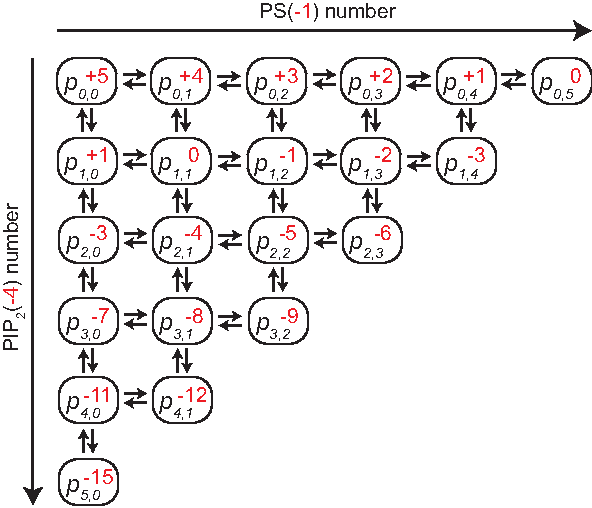
\includegraphics{../figures/peptide_complexes.pdf}
\end{center}
\caption[Transitions between PLCs]{Transitions between the peptide complexes $p_{i,j}$ (black arrows) and their total charge (in red), depending on the number of PS and PIP$_2$ bound to the peptide.}
\label{fig:peptide_complexes}
\end{figure}

It was hypothesized that any transition between PLCs in Fig. \ref{fig:peptide_complexes} can be described by a kinetic equation (see \eqref{er_p00}--\eqref{er_p05}). This assumption can be tested by constructing a system of kinetic equations between PLCs and validating its results against the MCA simulation data. I will call a transition between two complexes as a peptide transition reaction (equivalent to an ionic reaction in chemistry) and it will appear as R$_{i,j}^p$ in the mass-action equations of the complexes.

\subsection{Peptide transition reactions on binary membranes}

As a simple case let us consider peptide transition reactions on binary membranes, consisting only of neutral PC and monovalent PS lipids (first row in Fig. \ref{fig:peptide_complexes}). In this case the peptides can only sequester PS lipids and their charges vary from +5 to 0. One can distinguish between 6 different PLCs: $p_{0,0}$, $p_{0,1}$, $p_{0,2}$, $p_{0,3}$, $p_{0,4}$, $p_{0,5}$. Since I describe a transition between two complexes by a kinetic equation, one can define kinetic constants that determine the rate of the transition. Let $k_{i,j}$ be an association constant of PS with $p_{i,j}$ PLC and $h_{i,j}$ be a dissociation constant of PS from $p_{i,j}$ PLC. Based on the diagram in Fig. \ref{fig:peptide_complexes} one can write a system of equations that describes peptide transition reactions on a binary membrane as follows:
\begin{equation}
 \label {er_p00}
 R_{0,0}^p=\frac{\partial p_{0,0}}{\partial t}=h_{0,1} \cdot p_{0,1} - k_{0,0}\cdot p_{0,0} \cdot c_1
\end{equation}
\begin{equation}
 \label {er_p01}
 R_{0,1}^p=\frac{\partial p_{0,1}}{\partial t}=k_{0,0} \cdot p_{0,0} \cdot c_1 + h_{0,2} \cdot p_{0,2} - k_{0,1} \cdot p_{0,1} \cdot c_1 - h_{0,1} \cdot p_{0,1}
\end{equation}
\begin{equation}
 \label {er_p02}
 R_{0,2}^p=\frac{\partial p_{0,2}}{\partial t}=k_{0,1} \cdot p_{0,1} \cdot c_1 + h_{0,3} \cdot p_{0,3} - k_{0,2} \cdot p_{0,2} \cdot c_1 - h_{0,2} \cdot p_{0,2}
\end{equation}
\begin{equation}
 \label {er_p03}
 R_{0,3}^p=\frac{\partial p_{0,3}}{\partial t}=k_{0,2} \cdot p_{0,2} \cdot c_1 + h_{0,4} \cdot p_{0,4} - k_{0,3} \cdot p_{0,3} \cdot c_1 - h_{0,3} \cdot p_{0,3}
\end{equation}
\begin{equation}
 \label {er_p04}
 R_{0,4}^p=\frac{\partial p_{0,4}}{\partial t}=k_{0,3} \cdot p_{0,3} \cdot c_1 + h_{0,5} \cdot p_{0,5} - k_{0,4} \cdot p_{0,4} \cdot c_1 - h_{0,4} \cdot p_{0,4}
\end{equation}
\begin{equation}
 \label {er_p05}
 R_{0,5}^p=\frac{\partial p_{0,5}}{\partial t}=k_{0,4} \cdot p_{0,4} \cdot c_1 - h_{0,5} \cdot p_{0,5}
\end{equation}

\subsection{Limitations of the peptide transition model}
\label{CM_peptide_limitations}

If the concentration of PLCs is comparable with the concentration of lipids ($c_1\sim p_{0,j}$) in the membrane then the following statements should be taken into account:
\begin{enumerate}
 \item Sequestration of lipids on PLCs changes the concentration of free membrane lipids in accordance with equation:
\begin{equation}
 \label {er_c1}
 R_1^l=\frac{\partial c_1}{\partial t}=\sum_{j=1}^{5} h_{0,j} \cdot p_{0,j} - \sum_{j=0}^{4} k_{0,j}\cdot p_{0,j} \cdot c_1 
\end{equation}

Thus, $R_1^l$ should be added to the lipid diffusion equation \eqref{system1}.

\item Since the PLCs consist of both peptide and lipids, their concentrations should be explicitly added to the membrane incompressibility restriction \eqref{restriction2}, to account for the lipids belonging to the PLCs.
\end{enumerate}

However, if one assumes that the concentration of PLCs is much smaller than the concentration of PS:
\begin{equation}
 \label{peptide_assumption1}c_1\gg p_{0,j}
\end{equation}
then peptide transition reactions do not significantly change the PS concentration and, therefore, the concentration of monovalent PS lipids is constant during the time of equilibration of peptide transition reactions:
\begin{equation}
 \label{peptide_assumption2}c_1 = \text{const}
\end{equation}

In turn, if eq. \eqref{peptide_assumption2} holds, then $R_1^l$ equals 0 during the time of equilibration and membrane incompressibility restriction \eqref{restriction2} does not have to be changed.

Since at relevant biological conditions eq. \eqref{peptide_assumption1} is typically satisfied (see Appendix \ref{appendix_concentration}), hereafter I solve the general system of equations \eqref{general_system} under the condition \eqref{peptide_assumption1}

\subsection{Peptide transition reaction constants}

\label{reaction_constants}

Values of association and dissociation constants $k_{0,j}$ and $h_{0,j}$ \eqref{er_p00}--\eqref{er_p05} are defined by obtaining the best fit between the probability density functions of the PS-peptide association in the CM and in the MCA (Fig. \ref{fig:occupation_probabilities}). To obtain the probability density functions in the CM one has to solve the system of ordinary differential eqs. \eqref{er_p00}--\eqref{er_p05} numerically (this can also be done by using various software packages, e.g. Matlab) or analytically (subsection \ref{analytical_electro_reaction}) on a uniform membrane. 

To minimize the parameter space, available for defining $k_{0,j}$ and $h_{0,j}$, a preliminary estimation of how $k_{0,j}$ and $h_{0,j}$ depend on system variables can be done as follows. Since it has been shown in the MCA that the peptide residues interact with the membrane lipids independently (subsection \ref{lipid_demixing}), one can define the elementary association and dissociation constants of a PS lipid, interacting with the peptide residue -- $k_{PS}$ and $h_{PS}$, so that the total constants $k_{0,j}$ and $h_{0,j}$ are proportional to the elementary ones:
\begin{equation}
 \label{electro_reaction_proportionality-1}k_{0,j}\sim k_{PS}; \hspace{1in} h_{0,j}\sim h_{PS};
\end{equation}

Additionally, the probability of the PS-PLC association, according to the combinatoric rules, is proportional to the number of vacant (not bound to a PS lipids) PLC residues and equals 0, when the PLC is fully occupied by PS. Analogously, the probability of the PS dissociation from the PLC is proportional to the number of occupied (bound to a PS lipids) PLC residues and equals 0, when the PLC is free of PS. Since the number of vacant positions is defined by the charge of the PLC ($z_{0,j}$), the arguments above can be include in the eq. \eqref{electro_reaction_proportionality-1} as follows:
\begin{equation}
 \label{electro_reaction_proportionality0}k_{0,j}\sim\frac{z_{0,j}}{z_{0,0}}k_{PS}; \hspace{1in} h_{0,j}\sim\Big(1 - \frac{z_{0,j}}{z_{0,0}}\Big)h_{PS};
\end{equation}

Finally, in the MCA the dissociation of PS from the peptide leads to a Kawasaki swap between the negatively charged PS and neutral PC, so that the PC occupies the position directly underneath the peptide residue, instead of the PS. In the case of the membrane fully occupied by PS (without PC lipids) the dissociation of the PS lipid from the peptide residues is impossible, since the Kawasaki swap of the lipids does not change the system configuration, making all peptide residues always occupied by PS lipids. To implement this phenomenon in the CM I assume that the dissociation constant $h_{0,j}$ is proportional to the concentration of neutral PC lipids ($c_3$) in the membrane plane. This assumption automatically vanishes $h_{0,j}$ if the concentration of PC is 0. Thus, the final forms of $k_{0,j}$ and $h_{0,j}$ are the following:
\begin{equation}
\label{electro_reaction_constants}
 k_{0,j} = \frac{z_{0,j}}{z_{0,0}}k_{PS}; \hspace{1in} h_{0,0} = \Big(1 - \frac{z_{0,j}}{z_{0,0}}\Big)\frac{c_3}{C_m}h_{PS}; 
\end{equation}

The elementary constant $h_{PS}$ can be estimated from the averaged association time $\tau$ of PS with the peptide (Fig. \ref{fig:lipid_association_times}), obtained in the MCA. On the binary membrane $\tau$ does not significantly change with the PC concentration and is about 10 iteration steps. Since the ``real'' time of one iteration step was defined as $\sim$0.1 $\mu$s (subsection \ref{testing_calibration_MCA}) the ``real'' association time of PS with the peptide can be chosen as $\tau$ = 1 $\mu$s. Assuming that the frequency of the dissociation events is normally distributed (mathematical analogy with a radioactive decay) the average dissociation constant $h_{PS}$ should be inversely proportional to $\tau$:
\begin{equation}
\label{elementary_dissociation}
 h_{PS}\sim\frac{1}{\tau}\approx 10^6 \hspace{0.1in} \frac{1}{\text{s}}
\end{equation}

\begin{figure}[!ht]
\begin{center}
 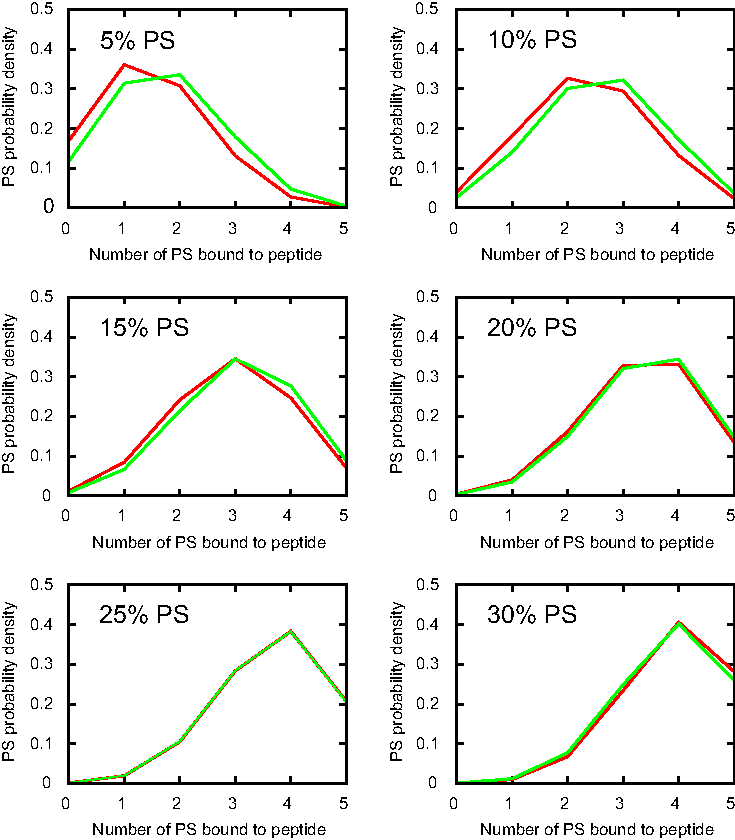
\includegraphics[scale=1.1]{../figures/occupation_probabilites_maraphet1.pdf}
\end{center}
\caption[Comparison of CM and MCA for the probability density functions of peptide-PS association]{Probability densities functions of PS association with the peptides at various concentrations of PS on a homogeneous membrane. Red line - results of the CM, green line - results of the MCA.}
\label{fig:occupation_probabilites1}
\end{figure}

I use this value of $h_{PS}$ in the solution of the CM with the following initial conditions (estimated in the Appendix \ref{appendix_concentration}): $p_{0,0}^0 = 100$ $\mu$M and the membrane concentration of PS varies from 0.015 M (5\% of $C_m$) to 0.09 M (30\% of $C_m$).  Solution of the system \eqref{er_p00}--\eqref{er_p05} provides values of PLCs concentrations, that are then normalized by the total peptide concentration $\sum_{j=0}^5p_{0,j}=p_{0,0}^0$. The best fit (Fig. \ref{fig:occupation_probabilites1}) between the peptide occupation probabilities in the CM and in the MC simulations is achieved for $k_{PS}$ = 2.7$\cdot 10^7$ $1/(M\cdot s)$ ($h_{PS}$ is defined in the eq. \eqref{elementary_dissociation}), using the least mean-square method. 

I use the values of $k_{0,j}$ and $h_{0,j}$, defined by eq. \eqref{electro_reaction_constants} with estimated values of $k_{PS}$ and $h_{PS}$, everywhere throughout the calculations in the CM. Note that these constants are derived for a binary membrane only, consisting of neutral PC and monovalent PS lipids. Addition of PIP$_2$ lipids to the membrane plane with the peptides requires recalculation of $k_{0,j}$ and $h_{0,j}$.

\subsection{PLCs contributions to free energy and fluxes}

\label{peptide_free_energy_contribution}

In the CM it is assumed that the PLCs are located in the same plane as membrane lipids. As discussed above (see subchapter \ref{CM_peptide_limitations}), under the assumption \eqref{peptide_assumption1}, the membrane incompressibility restriction \eqref{restriction2} is not imposed on the PLC dynamics. Since PLCs diffuse in the membrane plane their entropic and internal energy contributions to the free energy will have the same forms as for lipids (eqs. \eqref{entropy_sum} and \eqref{internal_energy_density}). Furthermore, the electrochemical potential of the PLCs also has the same form \eqref{chemical_potential_extended} except for the Lagrange multiplier:
\begin{equation}
\label{elchempot_prot}\frac{\mu_{0,j}}{k_BT}= \frac{\mu_{0,j}^{0}}{k_BT} + \log p_{0,j} + z_{0,j}\psi
\end{equation}

I assume that due to their low concentrations all PLCs diffuse freely and that there are no cross diffusion effects in their dynamics. Then Fick's first law is applicable to the PLCs and the flux of the $j^\text{th}$ PLC is defined similar to \eqref{flux_lipid}:
\begin{equation}
 \label{flux_prot}\vec{\mathbf{J}}_{0,j}=-D_{0,j}(\vec{\mathbf{\nabla}} p_{0,j} + z_{0,j} p_{0,j} \vec{\mathbf{\nabla}}\psi)
\end{equation}

\subsection{Average total and effective charges of the peptides}

\label{total_effective_charge}

If all PLCs have the same diffusion coefficients $D^p$, then eq. \eqref{flux_prot} allows one to calculate the total average electro-flux (considering only the part with the electrostatic potential $\psi$) of the peptides on the membrane:
\begin{equation}
\label{flux_prot_tot1}\vec{\mathbf{J}}_{tot}=\sum_{j=0}^5 \vec{\mathbf{J}}_{0,j}=-D^p\sum_{j=0}^5 z_{0,j} p_{0,j} \vec{\mathbf{\nabla}}\psi
\end{equation}

The sum $\sum_{j=0}^5 z_{0,j} p_{0,j}$ in the eq. \eqref{flux_prot_tot1}, normalized by the total peptide concentration $P_{tot} = \sum_{j=0}^5 p_{0,j}$, is equivalent to the total peptide charge obtained in the MCA (Fig. \ref{fig:total_peptide_charge}):
\begin{equation}
 \label{Z_tot}Z_{tot} = \frac{\sum_{j=0}^5 z_{0,j} p_{0,j}}{P_{tot}}
\end{equation}

Solution of the system \eqref{er_p00}--\eqref{er_p05} (see subsection \eqref{reaction_constants}) on the membrane with different PS compositions provides the dependence of $Z_{tot}$ \eqref{Z_tot} on the membrane concentration of PS. Comparison of the total average charge of the peptides in the CM and in the MCA (Fig. \ref{fig:total_effective_charge}) shows that the peptide transition reaction system \eqref{er_p00}--\eqref{er_p05} faithfully describes the reduction of the peptide total charge with the lipid membrane concentration and is in agreement with the MCA results. Note that fig. \ref{fig:total_effective_charge} is similar to fig. \ref{fig:effective_peptide_charge}.

\begin{figure}[!ht]
\begin{center}
 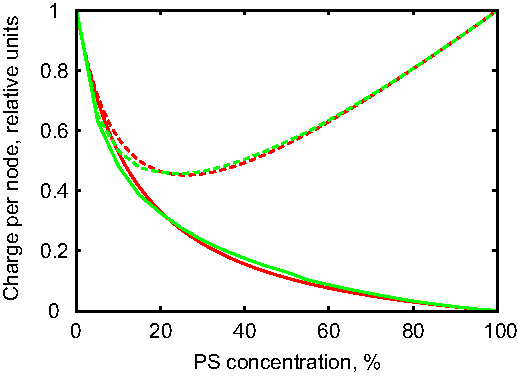
\includegraphics[scale=1.0]{../figures/total_effective_charge_maraphet.pdf}
\end{center}
\caption[Average total and effective charges of the peptides in CM and in MCA]{Average total and effective charges of the peptides in the CM (red) and in the MCA (green). Solid lines correspond to the total charges, dashed lines correspond to the effective charges.}
\label{fig:total_effective_charge}
\end{figure}

However, as it was shown in the MCA, the velocity of the peptide on a gradient of monovalent lipids is determined not by the total peptide charge, but by the effective charge associated with the translocating peptide (chapter \ref{description_peptide_effective_charge}), which has the following form (per one peptide residue, eq. \eqref{effective_charge}):
\begin{equation}
\label{effective_charge_CM}
 Z^{\text{eff}} = 1-p(\rho) + p(\rho)\cdot \rho
\end{equation}
where $\rho$ is a molar fraction of PS and $p(\rho)$ is the probability of the peptide residue being associated with PS.

In a similar way, in the CM the effective charge can be defined for each PLC. Since $1-p(\rho)$ is equivalent to the charge of the PLC ($z_{0,j}$) and the probability of association of the peptide residue with PS, $p(\rho)$, is equivalent to the number of the free residues in the PLC ($5 - z_{0,j}$), the effective PLC charge has the following form:
\begin{equation}
 \label{z_eff}z_{0,j}^{\text{eff}} = z_{0,j} + (5 - z_{0,j})\rho
\end{equation}

Thus, the effective average electro-flux of the peptides on the membrane (similar to the eq. \eqref{flux_prot_tot1}) has the following form:
\begin{equation}
\label{flux_prot_eff}\vec{\mathbf{J}}_{tot}=-D^p\sum_{j=0}^5\Big(z_{0,j} + (5 - z_{0,j})\frac{c_1}{C_m}\Big) p_{0,j} \vec{\mathbf{\nabla}}\psi
\end{equation}
where $c_1$ is the PS concentration and $C_m$ is the total concentration of the membrane plane. Therefore the average effective charge of the peptides can be written as:
\begin{equation}
 \label{Z_tot_eff}Z^{\text{eff}} = \frac{\sum_{j=0}^5 \big(z_{0,j} + (5 - z_{0,j})\frac{c_1}{C_m}\big) p_{0,j}}{P_{tot}}
\end{equation}

Again, solution of the system \eqref{er_p00}--\eqref{er_p05} on the membrane with different PS compositions provides the dependence of $Z^{\text{eff}}$ \eqref{Z_tot_eff} on the membrane concentration of PS. Comparison of the two approaches (Fig. \ref{fig:total_effective_charge}) shows that the correction \eqref{z_eff} of the PLC charge in the CM effectively accounts for the growth of $Z^{\text{eff}}$ at high PS concentrations, obtained in MCA, and that both approaches are in a good agreement.

I include the correction \eqref{z_eff} in the CM calculations. Thus, adding this correction in the equation of the PLC flux \eqref{flux_prot}  and using the continuity equation \eqref{continuity_equation}, one can define a diffusion equation describing the dynamics of PLCs on the membrane:
\begin{equation}
\label{protein_diffusion_equation}
 \frac{\partial p_{0,j}}{\partial t}=\vec{\mathbf{\nabla}} \Big(D_{0,j}\Big[\vec{\mathbf{\nabla}} p_{0,j} + \Big(z_{0,j} + (5 - z_{0,j})\frac{c_1}{C_m}\Big) p_{0,j} \vec{\mathbf{\nabla}}\psi\Big]\Big)
\end{equation}


\subsection{General form of membrane dynamics equations}

Combining together eq. \eqref{system1} with interconversion terms $K_i$ (eq. \eqref{krc1}) for lipid dynamics, eq. \eqref{protein_diffusion_equation} with peptide transition reactions $R_{0,j}^p$ (eqs. \eqref{er_p00}--\eqref{er_p05}) and assumption \eqref{peptide_assumption1} for small concentration of PLCs, and Poisson-Boltzmann equation \eqref{poisson-boltzmann1} with an additional term for PLCs (similar to the term describing lipid contribution -- see subsection \ref{peptide_free_energy_contribution}), one can write a general form of diffusion equations describing the spatio-temporal dynamics of lipids and PLCs on the binary membranes:
\begin{align}
\label{general_system}
\frac{\partial c_i}{\partial t}&=\vec{\mathbf{\nabla}} \Bigg(D_i\Big[\Big(\vec{\mathbf{\nabla}} c_i - c_i\frac{\sum_{j=1}^3 D_j\vec{\mathbf{\nabla}} c_j}{\sum_{j=1}^3 D_j c_j}\Big) + c_i \vec{\mathbf{\nabla}}\psi\Big(z_i - \frac{\sum_{j=1}^3 D_j z_j c_j}{\sum_{j=1}^3 D_j c_j}\Big)\Big]\Bigg) + K_{i} \nonumber \\
\frac{\partial p_{0,j}}{\partial t}&=\vec{\mathbf{\nabla}} \Big(D_{0,j}\Big[\vec{\mathbf{\nabla}} p_{0,j} + \Big(z_{0,j} + (5 - z_{0,j})\frac{c_1}{C_m}\Big) p_{0,j} \vec{\mathbf{\nabla}}\psi\Big]\Big) + R_{0,j}^p \nonumber \\
\vec{\mathbf{\nabla}}^2 \psi&=\frac{1}{\lambda^2}\sinh(\psi) - \frac{e^2 N_A}{k_B T\varepsilon\varepsilon_0} \sum_{i=1}^3 z_i c_i - \frac{e^2 N_A}{k_B T\varepsilon\varepsilon_0} \sum_{j=0}^5 z_{0,j} p_{0,j}
\end{align}